\chapter{Use Cases}\label{ch:cases}
As already mentioned, the system developed aims to deliver real-time performances also when used in real-world applications. Furthermore, the system provides some easy-to-embed APIs in order to be easily integrated in a full SLAM pipeline. Therefore, in this Chapter we provide two front-end systems developed in the \hyperref{http://labrococo.dis.uniroma1.it/}{}{}{Ro.Co.Co.Lab.} at Sapienza University that actually use this work as their back-end. In both cases, our system is used to perform 3D \textit{pose-graph} optimization.

\section{ProSLAM}\label{sec:proslam}
The work of Schlegel \textit{et al.} \cite{schlegel2017proslam} presents a stereo-visual system capable of mapping dynamic large-scale environments called ProSLAM. The system is designed with simplicity and modularity in mind and, thus, it is easy to implement and to understand also from people who are not Computer Vision or SLAM experts.

This works is also almost entirely self-contained and employs only a minimal set of external libraries - among which there is the library described in this work.

ProSLAM, despite its simplicity, is able to provide results comparable to other more complex state-of-the-art front-ends. Its goal is to generate a 3D map from the processing of a sequence of stereo-images. The map is intended as a collection of \textit{landmarks} - salient 3D points in the world characterized in its appearances by a unique descriptor - together with the camera trajectory. 

Landmarks acquired in a nearby region define a \textit{local map}; each local map constitutes a node of the graph - i.e. a $SE(3)$ transformation matrix. Edges between local maps encode the spatial constraints correlating local maps close in space. Those constraints are generated by two kind of events:

\begin{enumerate}
    \item \textbf{Tracking} of the camera motion between temporal subsequent maps;
    \item \textbf{Alignment} of local maps acquired at distant times as a consequence of \textit{relocalization} events - i.e. \textit{loop-closures}.
\end{enumerate}

Re-localization is more complex to address with respect to tracking. In fact, to achieve this goal it is necessary to compare descriptors of all the local-maps. This is an expensive operation, and it is efficiently performed by the \textit{Hamming Binary Search Tree} (HBST) \cite{schlegel2016hbst} library. The system periodically triggers graph optimization and this helps also the re-localization process.

It is good to notice that ProSLAM runs on \textit{single thread}, delivering performances comparable with other more complex and multi-thread systems - e.g. ORB-SLAM2 \cite{mur2017orb-slam2}.

\section{ProSLAM\_stud}\label{sec:froslam}
Colosi \textit{et al.} propose in their work ProSLAM\_stud \cite{colosi2017froslam} a further iteration on minimalism from original ProSLAM. It is a \textit{Master thesis} work, therefore its approach is more didactic than the original one. However, the system still delivers quite good performances both in terms of speed and accuracy. 

This systems embeds a new \textit{tracking} method based on KD-Tree that is able to provide a boost in speed with respect to ProSLAM, at the cost of little loss in accuracy.

ProSLAM\_stud keeps the single-treaded implementation and despite the minimal approach, it can push up to more than 80Hz - on average.

\section{KITTI Dataset}\label{sec:kitti}
Both ProSLAM and ProSLAM\_stud have been tested on two sequences of the KITTI dataset \cite{geiger2012kitti}. All the 22 available sequences, have been acquired using a car equipped with several sensors - e.g. stereo-cameras, Velodyne laser scanner and localization system that combines data from GPS, GLONASS and IMU - all calibrated and synchronized. 

\begin{figure}[!htb]
    \centering
    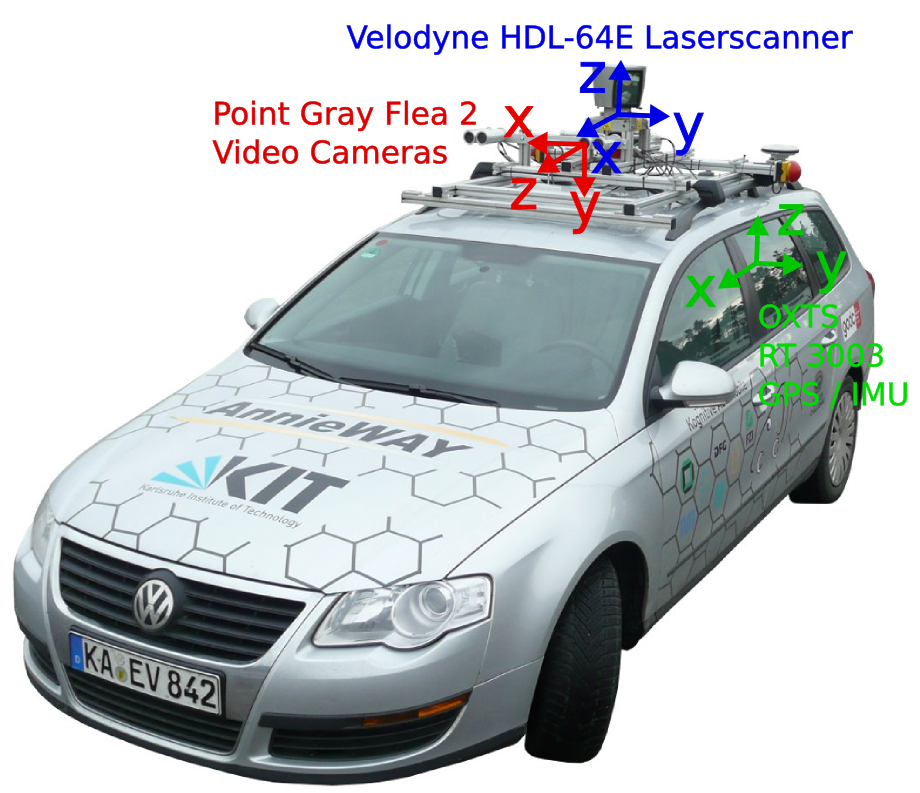
\includegraphics[width=0.5\textwidth]{figures/06_use_cases/kitti_setup.png}
    \caption{\textbf{KIT AnnieWAY acquisition method.} The KITTI dataset is acquired using an autonomous driving car, equipped with several sensor: a stereo-rig of high resolution cameras, Velodyne 3D laser scanner and a localization unit based on GPS/GLONASS/IMU.}
    \label{fig:kit_annieway}
\end{figure}

Clearly, the selected sequences are the ones with most loop-closures, in order to highlight the benefits of the optimization process. Figure \ref{fig:froslam_kitti} proposes a qualitative comparison of the performances using ProSLAM in sequences 00 and 06 respectively. 

\begin{figure}[!hbt]
    \centering
    \begin{minipage}[t!]{0.9\textwidth}
        \centering
        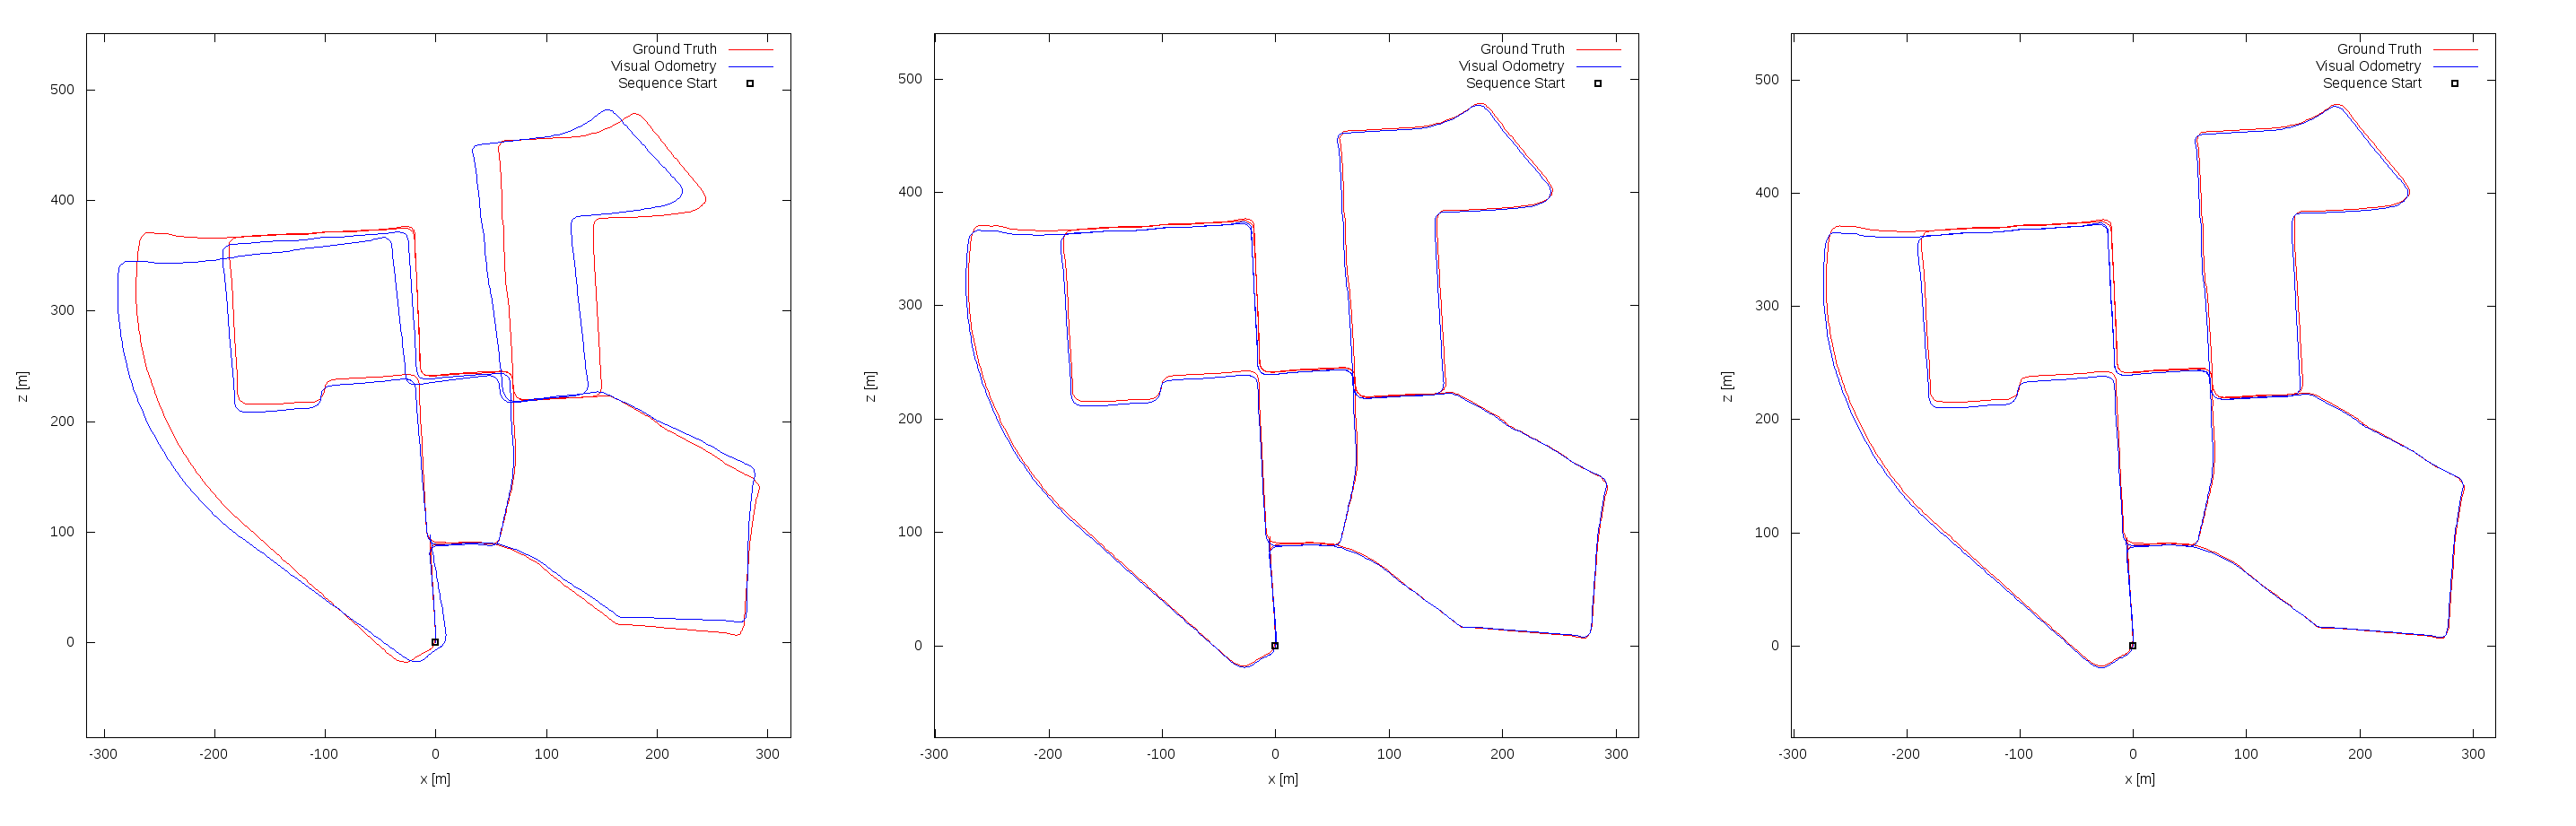
\includegraphics[width=\textwidth]{figures/06_use_cases/00_froslam.png}
        \label{fig:froslam_kitti_00}
    \end{minipage}\\
    \begin{minipage}[t!]{0.9\textwidth}
        \centering
        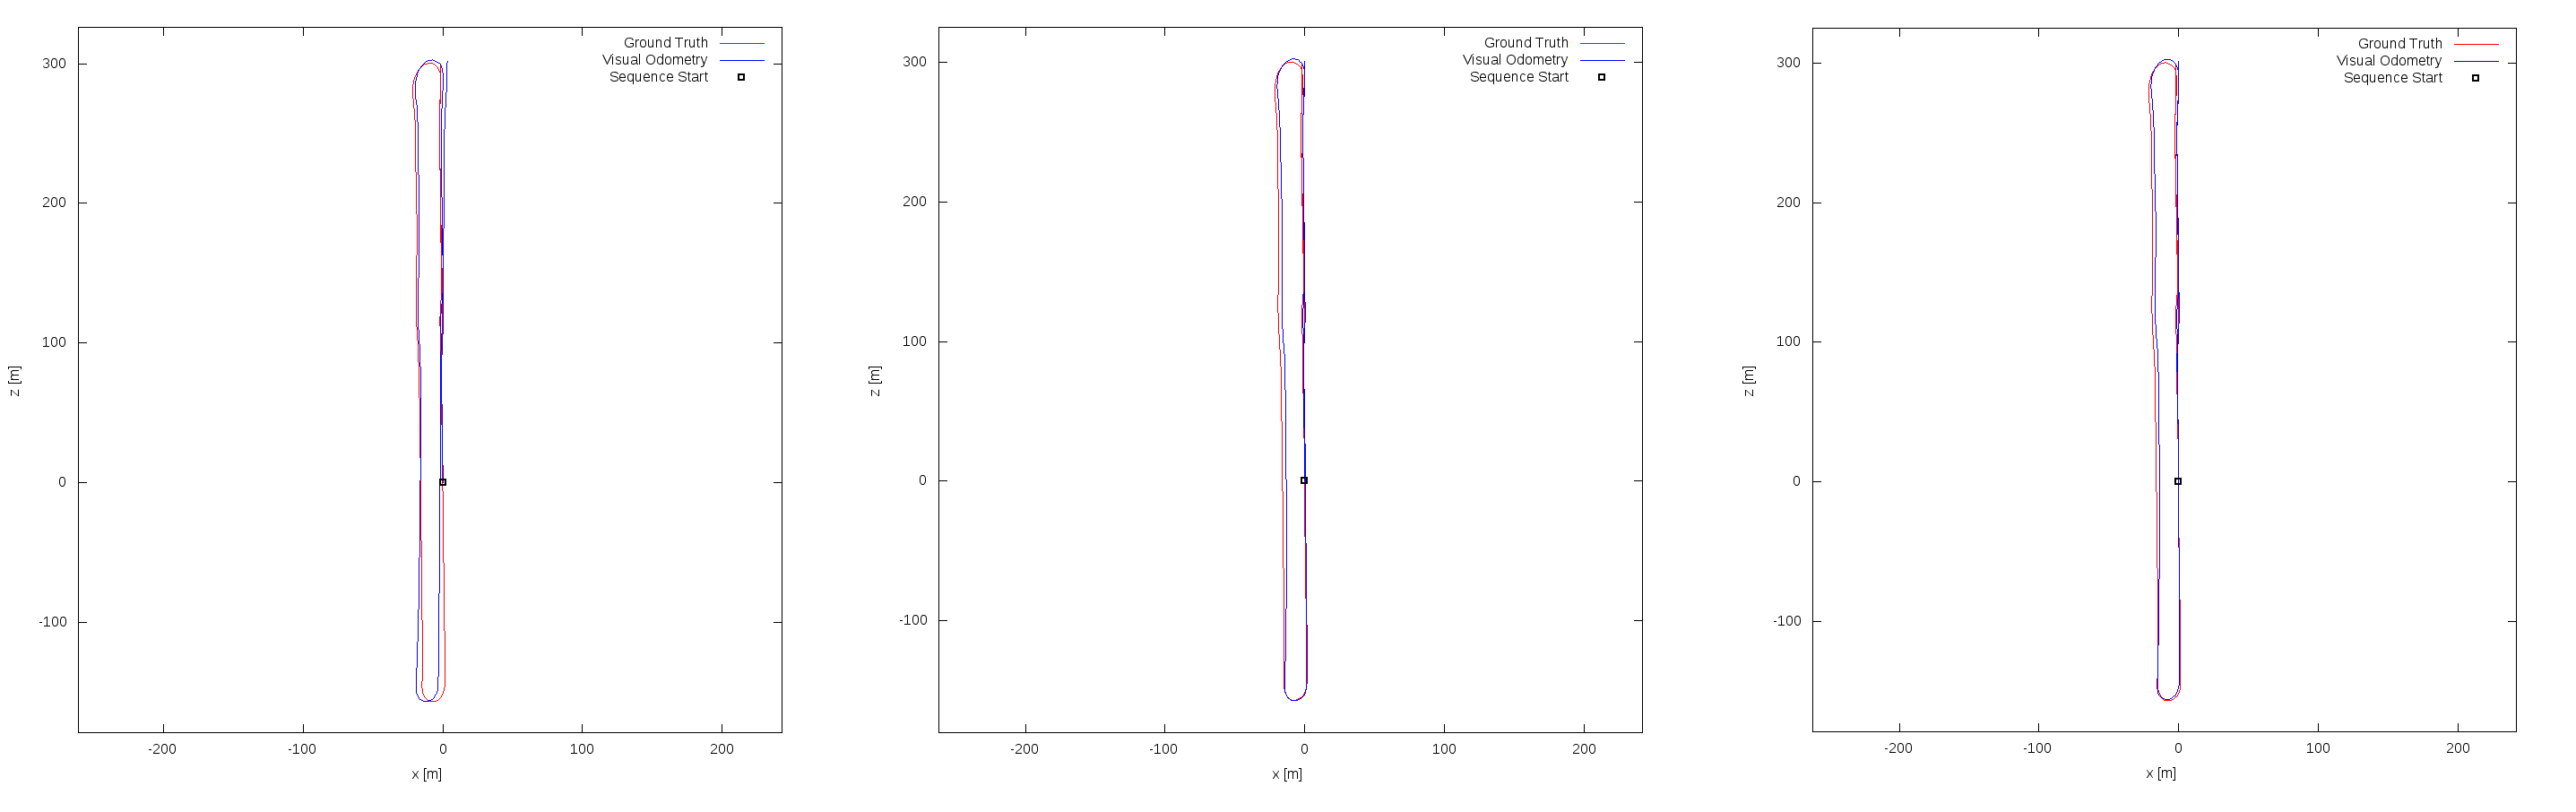
\includegraphics[width=\textwidth]{figures/06_use_cases/06_froslam.png}
        \label{fig:froslam_kitti_06}
    \end{minipage}%
    
    \caption{\textbf{ProSLAM results.} Starting from the top image it is proposed a comparison between the estimated and the real camera trajectory of sequence 00 - respectively in \textit{blue} and in \textit{red}. Proceeding from left to right it is proposed the estimation with \textit{no map optimization}, using \texttt{g2o} and using \textit{our approach} as optimizer. In the bottom image it is shown the same comparison but using sequence 06.} 
    \label{fig:froslam_kitti}
\end{figure}

\noindent The reader might already notice that the estimated trajectory is more consistent using a back-end that performs graph optimization; the figure also show how well our approach performs the optimization compared with another state-of-the-art system - i.e. \texttt{g2o} \cite{kummerle2011g}.

\begin{table}[!h]
    \centering
    \begin{tabular}{ l l l l l }
        \toprule 
        \multicolumn{5}{ c }{\textbf{ProSLAM Trajectory Error Evaluation}} \\ \hline
        Config & \multicolumn{2}{ c }{Sequence 00} &  \multicolumn{2}{ c }{Sequence 06} \\
        & Rotation $\left[\:\nicefrac{\deg}{100m}\right]$ & Translation $[\%]$ & Rotation $\left[\:\nicefrac{\deg}{100m}\right]$ & Translation $[\%]$\\
        \midrule
        OL & 0.397155 & 1.117624 & 0.393365 & 0.861104 \\ 
        \texttt{g2o} & 0.301858 & 0.731966 & 0.224632 & 0.733721 \\ 
        our & 0.272738 & 0.723581 & 0.219253 & 0.664294 \\ \hline
    \end{tabular}
    \caption{\textbf{ProSLAM Trajectory Error.} In this Table are reported the \textit{translation} and \textit{rotation} error of the final trajectory on both sequences. The contribution of a map optimizer is undeniable, however, the reader might appreciate the results obtained with our minimalistic approach, which are not far from the one obtained using the state-of-the-art system \texttt{g2o}.}
    \label{tab:proslam_results}
\end{table}

\noindent Furthermore, in Table \ref{tab:proslam_results} are proposed quantitative results about the final trajectory's error for each map optimizer used: the reader might appreciate the closeness of our approach with the \texttt{g2o}.

The same considerations can be made also using ProSLAM\_stud system, as depicted in Figure \ref{fig:froslam_stud_kitti} and in Table \ref{tab:proslam_stud_results}.

\begin{figure}[!hbt] 
    \centering
    \begin{minipage}[t!]{0.9\textwidth}
        \centering
        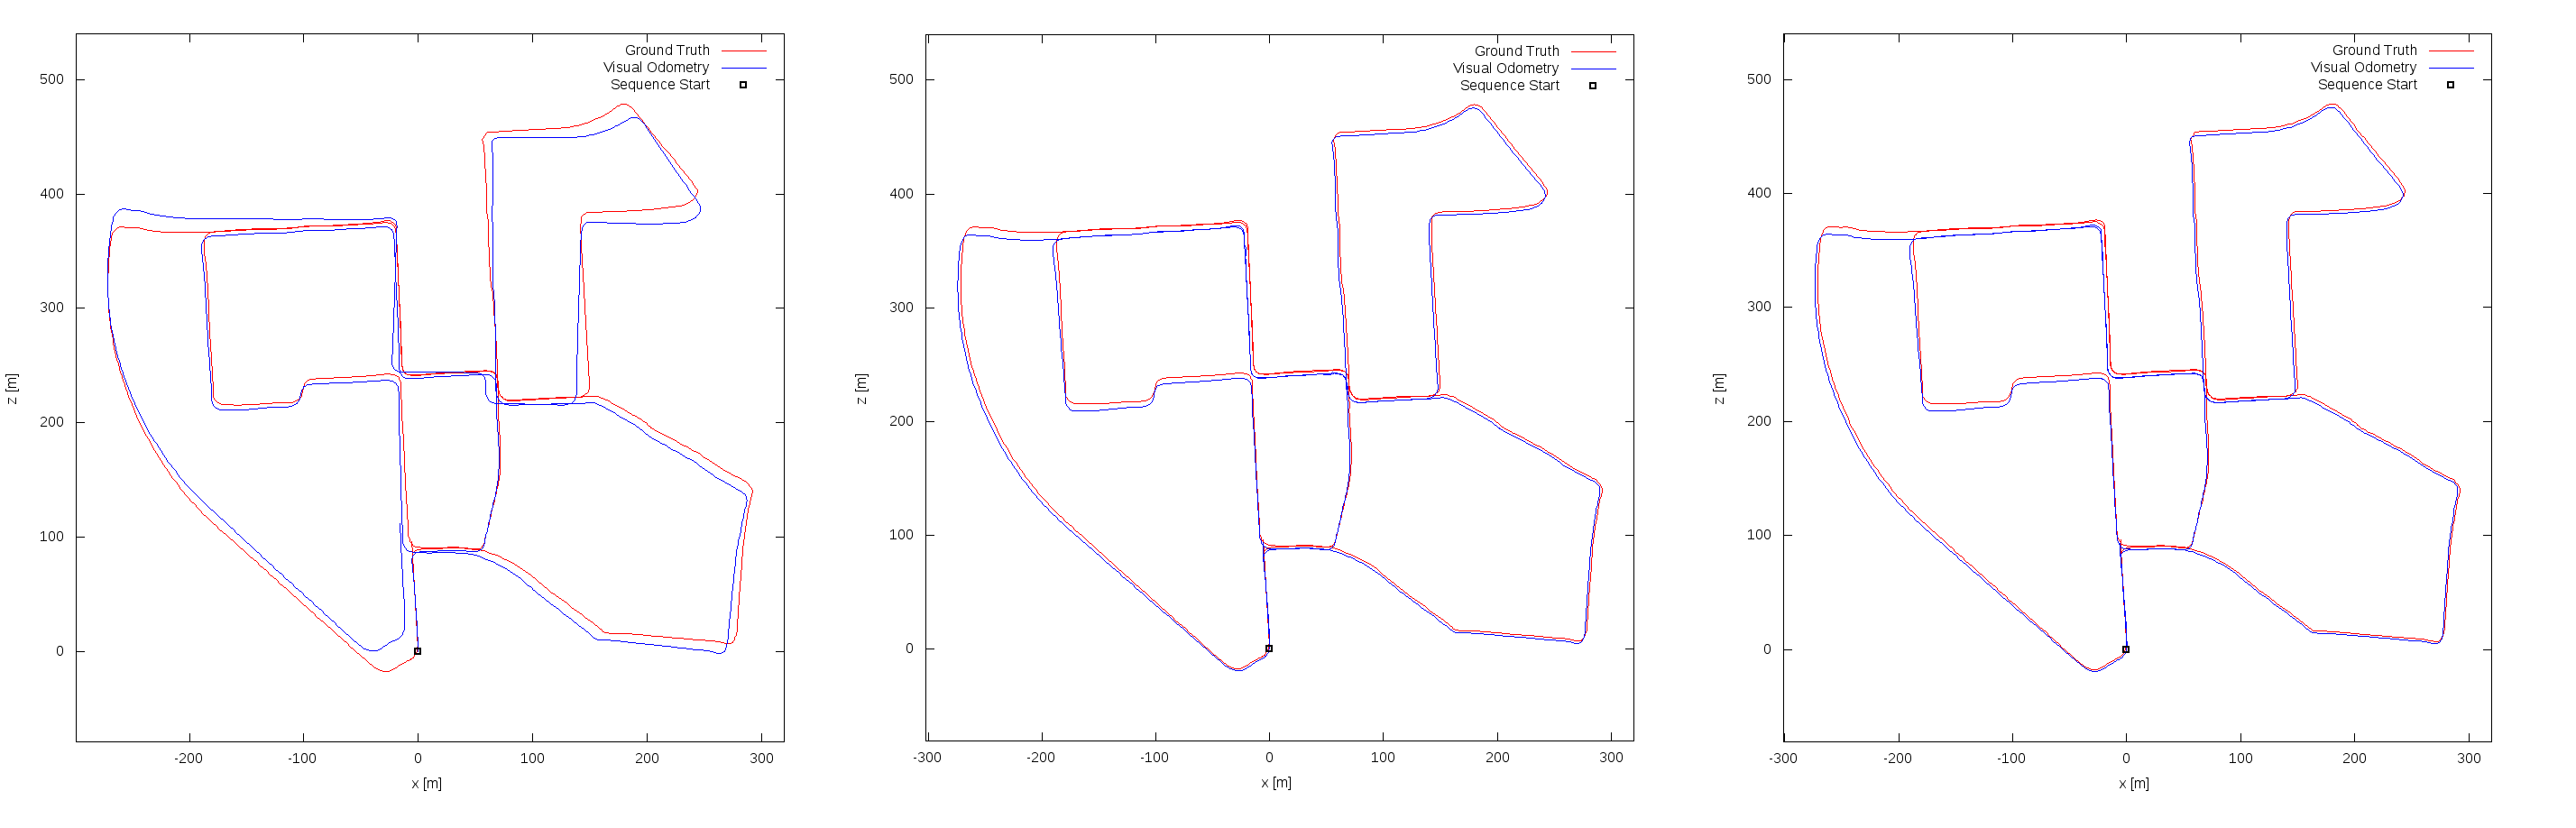
\includegraphics[width=\textwidth]{figures/06_use_cases/00_froslam_stud.png}
        \label{fig:froslam_stud_kitti_00}
    \end{minipage}\\
    \begin{minipage}[t!]{0.9\textwidth}
        \centering
        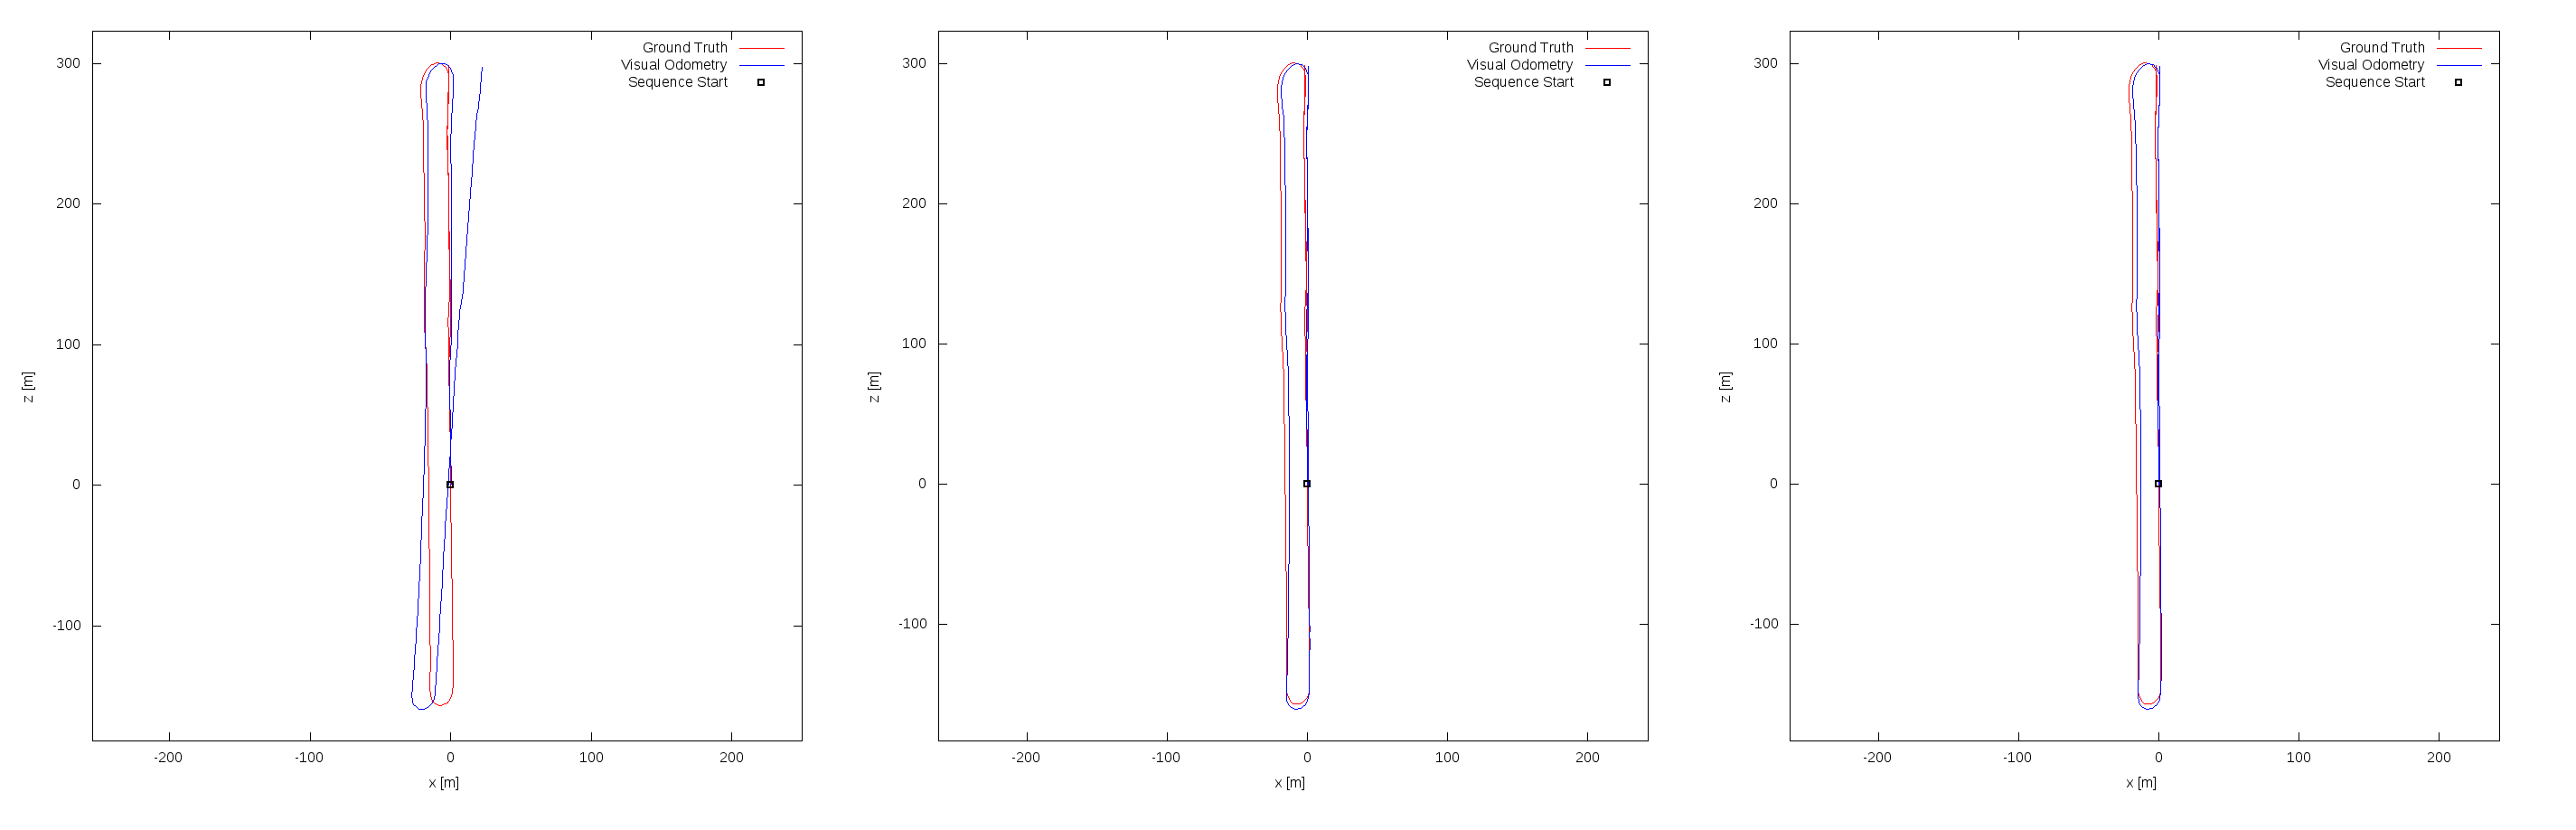
\includegraphics[width=\textwidth]{figures/06_use_cases/06_froslam_stud.png}
        \label{fig:froslam_stud_kitti_06}
    \end{minipage}%
    
    \caption{\textbf{ProSLAM\_stud results.} The top image proposes the estimated and real camera trajectory of sequence 00 - respectively in \textit{blue} and in \textit{red}. Again it is proposed the comparison between open-loop estimation, \texttt{g2o} and our approach. In the bottom image it is shown the same comparison but using sequence 06.} 
    \label{fig:froslam_stud_kitti}
\end{figure}

\begin{table}[!h]
    \centering
    \begin{tabular}{ l l l l l }
        \toprule 
            \multicolumn{5}{ c }{\textbf{ProSLAM\_stud Trajectory Error Evaluation}} \\ \hline
            Config & \multicolumn{2}{ c }{Sequence 00} &  \multicolumn{2}{ c }{Sequence 06} \\
            & Rotation $\left[\:\nicefrac{\deg}{100m}\right]$ & Translation $[\%]$ & Rotation $\left[\:\nicefrac{\deg}{100m}\right]$ & Translation $[\%]$\\
        \midrule
            OL & 0.615349 & 1.285283 & 0.745911 & 1.036123 \\ 
            \texttt{g2o} & 0.452409 & 0.941609 & 0.259771 & 0.785845 \\ 
            our & 0.357097 & 0.850793 & 0.272893 & 0.794151 \\ \hline
    \end{tabular}
    \caption{\textbf{ProSLAM\_stud Trajectory Error.} In this Table are reported the \textit{translation} and \textit{rotation} error of the final trajectory on both sequences. Even in this case, our approach delivers consistent results.}
    \label{tab:proslam_stud_results}
\end{table}

From this quantitative and qualitative analysis it is clear the contribution of a good back-end in the SLAM pipeline. Furthermore, they highlighted the quality reached by our system in real-world scenarios, delivering fast and accurate estimation despite it simplicity and minimalism.